\documentclass[10pt,twocolumn]{article}
\usepackage[letterpaper,margin=0.78in,columnsep=0.26in]{geometry}
\usepackage[T1]{fontenc}
\usepackage{lmodern,microtype,amsmath,amssymb,amsthm,booktabs,array,tabularx,xurl,graphicx}
\usepackage[numbers,sort&compress]{natbib}
\usepackage{tikz}
\usetikzlibrary{arrows.meta,positioning,fit}
\usepackage[hidelinks]{hyperref}
\usepackage{fancyhdr,caption}
\captionsetup{font=small,labelfont=bf}
\pagestyle{fancy}\fancyhf{}
\fancyhead[L]{\small Witness-CL}\fancyhead[R]{\small Research manuscript, September 2026}
\fancyfoot[C]{\thepage}\setlength{\headheight}{14pt}
\setlength{\emergencystretch}{2em}
\newtheorem{proposition}{Proposition}
\newtheorem{definition}{Definition}
\newcommand{\E}{\mathbb{E}}
\newcommand{\ind}{\mathbf{1}}
\newcommand{\code}[1]{\texttt{\small #1}}
\title{\vspace{-1.2em}\textbf{Witness-CL Technical Report:\\Constructive Contracts and Historical Evidence}}
\author{Samuel Mausberg}
\date{September 2026}
\hypersetup{pdftitle={Witness-CL Technical Report: Constructive Contracts and Historical Evidence},pdfauthor={Samuel Mausberg}}
\begin{document}\raggedbottom\maketitle
\begin{abstract}
A deployed agent should improve from its own experience while preserving useful
earlier behavior. We study why this requires more than accumulating memory or
accepting a checked update. Witness-CL combines executable learning mechanisms
with explicit contracts for evidence retention, model coverage, policy
continuations and exploration cost. Under supplied finite models, resets and
unchanged routing, these contracts preserve incumbent value and bound cumulative
exploration deficit. Online neural isolation preserves routed old functions,
while representation growth requires replaying observations that were redundant
in the old hypothesis class.

Controlled experiments reveal both useful learning and its limits. Reusing
learned features improves reward by 12.2 percentage points over a matched
no-reuse learner within a supplied grammar. Under a common query budget,
however, that learner attains 47.44\% final reward against 100\% for simple
history controls. Model-generated SQL exposes a different failure: a program
can reconstruct its source answer while the reconstruction ignores the program.
We implement bounded repair and a paid empty-relation intervention, and provide
a Lean counterexample showing why finite reconstruction plus dependence still
does not establish transfer. On a GH200, a 45-minute follow-up admits five
relations but never executes the checked reuse path before its deadline. Stored
guards sometimes answer fresh queries; warm qualification does not prevent
stale scalar errors. Retention panels remain incomplete. The resulting case study identifies concrete computational,
statistical and representation barriers, with source-linked experiments and
conditional proofs. It motivates a falsifiable delayed-corroboration mechanism.
General stateful-benchmark superiority and unrestricted no-forgetting remain
unestablished.
\end{abstract}

\section{The missing result}
An online agent can retain every byte of a successful interaction and still
perform worse later: retrieval may select irrelevant evidence, compression may
drop a convention, or a check may consume the last tool call needed to solve the
task. Conversely, a capable model can answer every question without learning
anything specific to the stream. The research target is therefore a conjunction:
experience must cause useful transfer, the complete system must beat competent
controls under a declared resource constraint, and protected old behavior must
remain adequate.

Continual Learning Bench (CL-Bench) makes this distinction concrete with
stateful-versus-stateless gain across six domains. Its evaluated full-context
ICL systems are strong controls \citep{asawa2026clbench}. AgentCL separately
shows the value of controlled compositional streams for diagnosing reuse
\citep{shu2026agentcl}. Neither benchmark's motivation licenses the universal
claim that memory systems never help. The question is which update mechanism
helps on which stream, at what cost, and with what regressions.

Witness-CL investigates a narrow candidate: learned, parameterized SQL
relations whose admission is supported by the agent's own executed observations.
Its SQL fixture exposes opaque names and a queryable documentation catalog,
allowing conventions to be learned across episodes. It is a custom mechanism
fixture, not a native CL-Bench result. This distinction matters because a single
catalog read can expose several conventions at once, and later direct SQL can
already attain the one-query floor.

This consolidated paper offers three bounded contributions. First, it makes
evidence retention, model coverage, continuation equality and exploration cost
explicit in executable controllers and checked conditional contracts. Second, it
measures representation learning, neural isolation, planning and feature reuse
against controls that expose their assumptions and costs. Third, it connects
model-generated program admissions to exact execution traces, repairs an
observed false admission and specifies the missing transfer test. The mechanisms
are related experimental systems, not one trained general-purpose agent. Useful
restricted results coexist with failed stronger comparisons; general benchmark
superiority and unconditional no-forgetting remain open.

\section{Learning and retention}
For the current SQL system, let $H_t$ be the agent's legal history through
episode $t$, $M_t$ its persistent state, and $\theta$ a fixed pretrained model.
Deployment updates are
\begin{equation}
 M_{t+1}=U_\theta(M_t,H_{t+1}),\qquad
 \pi_t=\pi_\theta(\cdot\mid M_t).
\end{equation}
For the current SQL agent, learning is nonparametric: program proposals, observations and memory
updates occur between episodes; model weights do not change. The absence of an
offline retraining phase does not make these updates free. $\pi_t$ includes
retrieval, prompts, decoding, routing, tool limits and fallback behavior.

For an episode instance $x$, let $A(\pi,x)\in\{0,1\}$ denote correctness and
$C(\pi,x)$ record SELECTs, model tokens, latency and retained bytes separately.
Define accuracy on a fixed distribution $D$ by
\begin{equation}
 V_D(\pi)=\E_{x\sim D,\,\xi}[A(\pi,x;\xi)],
\end{equation}
where $\xi$ includes solver randomness. A deployment gain compares the learned
state against the same backbone with its state reset, on matched instances and
resource rules. A positive gain alone does not show an advantage over full
history. Costs are reported jointly with accuracy; an unequal-accuracy token
table cannot establish matched-accuracy efficiency.

\begin{definition}[Scoped retention]
Choose a protected reference policy $\pi_{\rm ref}$, distributions
$D_1,\ldots,D_K$, allowed losses $\varepsilon_k\geq0$, and error probability
$\alpha$ before evaluation. A distributional retention claim requires
\begin{equation}\label{eq:retention}
 \Pr\!\left[\forall t,k:\,
 V_{D_k}(\pi_t)\geq V_{D_k}(\pi_{\rm ref})-\varepsilon_k\right]
 \geq 1-\alpha.
\end{equation}
\end{definition}
This is stronger than a final-checkpoint result, but weaker than a pointwise
claim about every realized task and random seed. Our experiments establish
neither. A frozen checkpoint evaluated once can support only that checkpoint's
specified distributional comparison. Repeated promotion requires a valid
lifetime error allocation; repeatedly accepting a small loss against the last
policy can accumulate a large loss against the original reference.

Preserving a program's bytes does not imply Eq.~\eqref{eq:retention}. Even
identical outputs do not protect reward when new checks change latency or
resource use. Under hidden concept drift, preserving an old answer can be wrong.
One must distinguish retaining competence on a fixed protected distribution
from adapting to a newly defined one.

\paragraph{Why a universal claim is unavailable.}
If two environments produce identical legal histories but require different
answers on a new question, an agent with that history must issue the same
answer distribution in both. It cannot guarantee correctness in both worlds.
For example, a zero-valued observation is consistent with different monetary
scales. This is an elementary identifiability boundary, not a claim that all
structured environments are unlearnable. Restrictions on tasks, informative
observations and explicit statistical assumptions are essential.

\section{Antecedents and the comparison we owe}
Executable reuse and iterative repair are established ideas. Voyager accumulates
executable skills and uses environment feedback to improve them
\citep{wang2023voyager}; Agent Workflow Memory induces reusable routines,
including during online interaction \citep{wang2024awm}. Dynamic Cheatsheet
retains transferable text and code \citep{suzgun2025dynamic}. Thus neither a
program library nor retries is our novelty claim.

ACE addresses information loss during context rewriting
\citep{zhang2025ace}; Evo-Memory's ReMem integrates reasoning, action and memory
refinement \citep{wei2025evomemory}; MemProbe combines interactions, insights and
skills \citep{shu2026agentcl}. These motivate controls that can retain working
SQL and exact documentation. Our old evolving-text arm is a particular
implementation, not a faithful replication of those algorithms.

Memento 2 formalizes reflected decision processes, while Memento-Skills uses
evolving external skills \citep{wang2025memento,zhou2026memento}. The former's
asymptotic connection to optimal behavior assumes local consistency of the LLM
near relevant cases and improving coverage; its policy-iteration and memory
convergence results impose additional conditions. Those premises do not supply
a finite-budget retention guarantee for this solver.

Neural memory and test-time weight adaptation provide a different axis.
Titans learns a neural memory mechanism \citep{behrouz2025titans}; end-to-end
test-time training updates on context through next-token prediction and
meta-trains updateability \citep{tandon2025ttt}. Their sequence-modeling results
are not evaluations of the present SQL policy. A frozen-backbone study cannot
establish superiority over these trained architectures. A later weight-update
comparison must hold available experience and total computation explicit.

High-confidence policy improvement and confidence sequences already provide
routes to statistical protection under sampling assumptions
\citep{thomas2015hcpi,howard2021confidence}. They do not discover useful
representations, make audit data free, or predict arbitrary future drift. Our
potential contribution lies in the measured connection from evidence to
computation to transfer, with these boundaries exposed.

Predictive state representations already model latent dynamics through
predictions of observable experiments \citep{singh2004psr}. Baseline
bootstrapping constrains policy changes with limited evidence
\citep{laroche2019spibb}, and DeepSPI couples representation/world-model
learning to safe online policy improvement \citep{delgrange2026deepspi}. Thus
our finite-class contracts are not a first solution to representation-aware
policy improvement. Their role is to expose exact coverage, continuation and
resource obligations in executable form.

For the SQL component, query-equivalence tools are a stronger antecedent than
instance agreement. SQLSolver proves supported equivalences using integer
arithmetic, while VeriEQL checks bounded database equivalence and can produce
counterexamples \citep{ding2023sqlsolver,he2024verieql}. We have not integrated
either. Their guarantees depend on supported syntax, constraints and modeled
SQL semantics; equivalence to an observed source query still does not prove
that the source answers the intended question.

\section{Evidence and execution contracts}\label{sec:contracts}
The earlier constructive systems answer a narrower question than the SQL
learner: what can be guaranteed when the environment family or a valid state
bound is supplied? Their value is to isolate the assumptions that disappear
when a language model must discover the representation itself. The following
contracts apply to those systems; they are not silently inherited by the
current SQL agent.

\subsection{Evidence must survive representation growth}
For a hypothesis class $\mathcal H$ and exact executed observations $E$, define
\begin{equation}
 \mathcal V(\mathcal H,E)=\{h\in\mathcal H:h\text{ agrees with every }e\in E\}.
\end{equation}
In a fixed finite class, keep an observation as a compact witness only when it
strictly shrinks the current version space. Induction gives the same final
version space as retaining every constraint, with at most
$|\mathcal H|-|\mathcal V|$ such witnesses. This equality does not require
realizability; retaining the true hypothesis additionally requires correct
feedback and its initial inclusion.

The qualification ``fixed class'' is essential. If new hypotheses $\mathcal G$
are introduced, the correct update is
\begin{equation}\label{eq:expansion}
 \mathcal V(\mathcal H\cup\mathcal G,E)
 =\mathcal V(\mathcal H,E)\cup\mathcal V(\mathcal G,E).
\end{equation}
Old constraints discarded as redundant on $\mathcal H$ can reject members of
$\mathcal G$. For example, if the old class contains only the constant-zero
rule, observing zero at input one removes nothing. A later rule predicting one
there is nevertheless inconsistent with that observation. Replaying only the
compact old witness set would admit it. Representation growth therefore stages
the enlarged class, replays complete original evidence and commits atomically.
An archive preserves the possibility of reinterpreting observations; it does
not certify that the enlarged class contains the true rule.

\subsection{Hidden dynamics with an exact partial-table cover}
A stronger implemented system assumes a stationary deterministic transducer
with at most $K$ hidden states, known finite action and output alphabets
$\mathcal A,\mathcal O$, and genuine episode resets. It observes executed
input/output traces, not hidden states or supplied transition tables. Public
objectives $g$ specify bounded reward functions of outputs. Policies are frozen
finite trees over observed output histories.

The learner maintains a union of partial transition tables. A defined edge
survives an observation only if its output agrees. An undefined visited edge
branches over its $K$ possible successor states while fixing the observed
output. End states are tracked inside an episode and discarded at reset;
identical partial tables are deduplicated. Every consistent complete table
follows one retained branch, and every retained completion agrees with the
observations. This is exact finite-class inference, not learned validity of the
state bound. Selecting a minimum-size fitted automaton would lose the coverage
property needed by the checker.

For candidate $p$, incumbent $b$ and current consistent class $C$, paired
symbolic execution computes
\begin{equation}\label{eq:robust}
 L_C(p,b;g)=\min_{m\in C}\{V_m(p,g)-V_m(b,g)\}.
\end{equation}
Both executions use the same unknown-edge assignments. A branch may close when
the complete remaining program, symbolic state and time agree; unread edges
then affect both continuations equally. Equality of the current action or
accumulated reward alone cannot justify closure. Exact residual-program keys
avoid equating unequal suffixes merely through a hash collision.

\begin{proposition}[Conditional incumbent preservation]\label{prop:incumbent}
Within a stationary era, suppose the actual transducer remains in every
complete class $C_n$, the programs and dispatch semantics are immutable, and
there is a separate incumbent $b_{n,g}$ for each public objective $g$.
Only a completed comparison with $L_{C_n}(p,b_{n,g};g)\geq0$ replaces that
objective's entry; all other entries remain unchanged. Then incumbent reset
value is nondecreasing for each protected public objective,
regardless of how an online neural or symbolic proposer changes.
\end{proposition}
\begin{proof}
Substitute the actual transducer into each universal inequality in
Eq.~\eqref{eq:robust}, then use transitivity across accepted replacements.
Class contraction preserves an earlier universal obligation. Class expansion
need not; it requires recertification and an explicitly new trust era.
\end{proof}
The preserved Lean statements formalize the implication from coverage and
bounds to retention. The full optimized Python search is not verified in Lean.
A work cap returns \code{UNKNOWN}, never a certificate from a truncated class.
An empty class returns inconsistency, avoiding vacuous certification.

This machinery is expensive. Along a paired path, at most
$u=\min(K|\mathcal A|,2H)$ previously unknown edges can be encountered.
Branching can reach $(K|\mathcal O|)^u$ assignments per partial table, before
cover and horizon overhead. A complete contingent policy tree can itself have
$\sum_{t=0}^{H-1}|\mathcal O|^t$ nodes. Common suffixes save work on particular
programs without making inference polynomial.

\paragraph{When full state is observable.}
The earlier supplied-model controller uses the stronger all-state condition
\begin{equation}
 r_m(t,s,c)+V_m^b(t+1,T_m(t,s,c))\geq V_m^b(t,s)
\end{equation}
for every live model, time and state, with $c=c(t,s)$. Backward induction then
replaces the old continuation value by the no-smaller candidate continuation,
yielding $V_m^c(t,s)\geq V_m^b(t,s)$ throughout the horizon. This is ordinary
Bellman policy improvement, formalized in \code{bellman\_improvement}. It is a
sufficient local condition; jointly beneficial changes can fail it. The later
hidden-state comparison instead checks complete policies from reset and must
not be described as establishing all-state improvement.

\subsection{Exploration has a separate contract}
An incumbent can be uninformative. Before executing an exploratory policy
$p_n$, the controller computes a nonrefundable debit
\begin{equation}
 d_n=\max\!\left(0,\max_{m\in C_n}
       [V_m(b_{n,g_n},g_n)-V_m(p_n,g_n)]\right).
\end{equation}
It executes only if cumulative debits remain within a declared $B$. Under the
same coverage, deterministic reset and reward assumptions,
\begin{equation}\label{eq:debit}
 \sum_{n=1}^N[V_{m^*}(b_{0,g_n},g_n)-R_n]
 \leq\sum_{n=1}^N d_n\leq B
\end{equation}
for every completed prefix. The first inequality follows episode by episode
from preservation of the incumbent for the executed objective and the worst-case
debit, with objective-specific reference $b_{0,g_n}$. Favorable outcomes
do not refund the announced debit.

Equation~\eqref{eq:debit} permits individual losses. It compares each execution
with a reference beginning at the same reset, not with the counterfactual
lifelong trajectory of a reference agent in a world with cross-episode effects.
Resetting the ledger at every detected regime does not establish one lifetime
bound. Unknown hidden drift can invalidate a certificate before feedback reveals
the change. These distinctions separate reward accounting from general safety.

\subsection{Protect the closed system, not just its module}
Let $F(z,u)$ be a full system transition, where $z$ includes controller memory,
routing, normalized inputs, permissions and environment state. If old and new
systems have equal $F(z,u)$ on a protected set $P$, and their common successor
remains in $P$, induction on the input tape gives equal output traces and final
states. The closure condition prevents a system from leaving the protected set
after one matching action and diverging later. The corresponding Lean contract
is \code{closed\_continuations\_equal}.

This is the precise reason that frozen modules can be useful but insufficient.
An unchanged module with a new router or input normalizer need not preserve the
old computation. The SQL runtime currently supplies neither a verified closed
state invariant nor the ordinary reference answer after a failed check.

\section{Learning representations and parameters}\label{sec:learning}
The repository contains several online update mechanisms. They
operate under different information contracts and must not be described as
one end-to-end trained language agent. The unifying design is to let a mutable
learner propose a change while a separate, explicit mechanism controls its use.
That division prevents a proposal score from becoming its own certificate.

\subsection{Projected residuals and their capacity cost}
An early parameter-learning component freezes feature map $\phi$ and predictor
$f$. If the columns of $U$ are an orthonormal basis for protected feature
vectors, set $P=I-UU^\top$ and train only $W$ in
\begin{equation}\label{eq:residual}
 f_W(x)=f(x)+WP\phi(x).
\end{equation}
For $\phi(x)\in\operatorname{span}(U)$, the residual is exactly zero for every
$W$. This is an algebraic fixed-feature result, related to orthogonal update
methods; it is not a guarantee for an arbitrarily changing nonlinear network
\citep{farajtabar2020ogd,lopezpaz2017gem}. Floating-point SVD and SGD give a
measured drift. The real-arithmetic residual using an approximate projector
is bounded by $\|W\|\,\|\widetilde P\phi(x)\|$; this does not bound
additional floating-point evaluation error. No complete rounding analysis or
bitwise real-arithmetic equality is claimed.

Protection consumes capacity. If protected vectors span the whole feature
space, $P=0$ and no residual update can change any output. For isotropic new
features and desired linear change $v^\top\phi$, the best possible residual
squared error is $\|U^\top v\|^2$: the protected component cannot be fitted.
This identifies when additional observable context or new isolated features
are necessary. It cannot resolve a conflict hidden from the input.

\subsection{Frozen learned modules and routing}
A separate neural experiment trains a new feature map and head online, then
freezes that module at registration. Earlier public-scope dispatch and input
construction stay fixed. This preserves old module functions exactly under
that routing contract, while consuming storage for additional modules.
Architectural isolation and reuse have direct antecedents in progressive
networks \citep{rusu2016progressive}; neither freezing nor a growing archive
is novel by itself.

The diagnostic uses two possible actions and exact binary success. Chosen
action plus success determines the binary target, so training does use real
feedback. That reduction fails for noisy success or more than two actions
without further supervision. These small neural modules are distinct from the
frozen language models in the SQL studies. Their historical results quantify
the isolation-versus-replay tradeoff in Section~\ref{sec:historical}.

\subsection{Numerical feature search with paid promotion}
The relational learner removes the enumerated world class but supplies an
84-feature grammar. Each observed SQLite join produces rows
$z_i\in\mathbb R^6$ and features
\begin{equation}
 \phi_m(z)=\sum_i\prod_{k=1}^6 z_{ik}^{m_k},\qquad
 m\in\mathbb N^6,\quad\|m\|_1\leq3.
\end{equation}
Reports are one- or two-term integer combinations in this grammar. The learner
receives a public report token, fixed table measurements and, only after its
ordinary prediction, the exact scalar target. It does not receive the hidden
formula. This is stronger feedback than the later SQL agent's correctness bit.

A growing learner begins with count and six linear sums. Once data outnumber
active features by two, it projects candidate columns off the current design,
scores residual correlation for at most 16 candidates, adds a feature and refits
scaled least squares. Each report has at most 12 features. Promoted nonlinear
syntax enters a shared bank of at most 32 features and changes search order on
later reports; coefficients still come from each report's own examples.
The no-reuse arm removes only bank priority. Three-step matching pursuit and
full 84-feature ridge on legal history are stronger simple controls.

This experiment learns feature selection and coefficients online, not new
operators. A fourth-degree parity on the complete sign cube is orthogonal to
every supplied degree-at-most-three monomial. No amount of auditing repairs
that representational misspecification. Irreversible early feature choices can
also fill the width cap before useful terms are selected. The move to
model-proposed SQL is motivated by these limits, without claiming that it has
already overcome them empirically.

\section{Statistical admission and its opportunity cost}\label{sec:statistical}
When a finite correct model class is unavailable, a frozen proposal can instead
be compared with an incumbent using fresh paired outcomes. For bounded rewards,
let $D_t=R_t(p)-R_t(b)\in[-1,1]$. With a predictable stake
$\lambda_t\in[0,1]$, the process
\begin{equation}\label{eq:eprocess}
 E_0=1,\qquad E_t=\prod_{i=1}^t(1+\lambda_iD_i)
\end{equation}
is a nonnegative supermartingale under
$\E[D_t\mid\mathcal F_{t-1}]\leq0$. Here $\mathcal F_0$ includes every
observation used to select the frozen comparison, and the filtration includes
all preceding training, selection and audit data. The conditional expectation
of each factor
is at most one. Ville's inequality bounds ever reaching $1/\alpha_j$ by
$\alpha_j$. Spending $\alpha_j=\alpha/[j(j+1)]$ over all started comparisons
bounds the probability of any false acceptance by $\alpha$, under the stated
conditional nulls \citep{waudby2024betting,howard2021confidence}. These are
standard statistical tools, not new concentration results.

For a claim about future policy value, fresh independent sampling from a
stationary protected distribution is a sufficient condition. A candidate,
incumbent, routing state or scope changed after seeing its audit data requires
a new valid comparison. Distinct sample identifiers alone cannot establish
freshness. Adaptive exact reuse of a hidden test set is also not justified by
calling it a holdout \citep{dwork2015holdout}.

The error allocation is per gate/run, not simultaneous over all experimental
arms and seeds. The implemented relational gate fixes $\lambda=1/2$, caps audits at 64 pairs,
and checks floating-point log wealth against exact rational capital for the
represented rewards. Every started audit spends its error allocation, even
when abandoned. Audit observations cannot enter fitting; promoted feature
syntax can influence later proposals, which require fresh audit data. Its
journal can detect inconsistent edits, but an unkeyed hash chain cannot
authenticate rewards or prevent a complete rollback without trusted external
state.

\subsection{Null validity does not imply useful power}
The first comparison receives $\alpha_1=.025$. A constant gain $d$ can pass
within 64 pairs only if $(1+d/2)^{64}\geq40$, or approximately
$d\geq.118664$. A constant five-point gain cannot pass this capped test.
Worse, consider independent $D=+1$ with probability $.55$ and $D=-1$ otherwise.
The mean gain is $.1$, but
\begin{equation}
 .55\log1.5+.45\log.5\approx-.08891<0.
\end{equation}
Moreover $.55\sqrt{1.5}+.45\sqrt{.5}<1$, so $\sqrt{E_t}$ is a nonnegative
supermartingale under this positive alternative. Its eventual crossing
probability is at most $\sqrt{\alpha_1}<.159$, even without a sample cap.
This is a power failure of the fixed large stake, not a violation of null
validity. A prespecified smaller bet, predictable variance-sensitive betting,
or a valid fixed mixture is a concrete standard alternative.

Statistical cost is not merely an implementation defect. In the independent
$\{-1,+1\}$ family with mean $\mu>0$, a sequential test with null admission
probability at most $a$ and power at least $1-b$ satisfies the standard
change-of-measure requirement
\begin{equation}\label{eq:kl}
 \E_\mu[N]\,\operatorname{kl}((1+\mu)/2\,\|\,1/2)
 \geq\operatorname{kl}(1-b\,\|\,a),
\end{equation}
for $0<a<1-b<1$ and a stopping time with finite expected duration under
the alternative; the terminal decision must be measurable at stopping. It
follows by the likelihood-ratio
chain rule and data processing to the final decision
\citep{kaufmann2016complexity}. At $a=.025$, $b=.2$ and $\mu=.05$, it requires
about 1964 expected informative observations. This restricted lower bound does
not cover every reward distribution; it explains why small noisy gains are
harder than nearly deterministic improvements.

\subsection{What Lean adds to statistical protection}
For a finite population of $C$ contexts, let $T(p)$ sum a policy's integer
returns in $[0,B_r]$. For accepted update $j$, define its actual violation
\begin{equation}
 F_j=\ind\{T(p_j)+\tau_j<T(p_{j-1})\},\quad\tau_j\geq0.
\end{equation}
The Lean accounting bridge proves
\begin{equation}\label{eq:promotion}
 T(p_0)\leq T(p_n)+\sum_j\tau_j+CB_r\sum_jF_j,
\end{equation}
and the analogous inequality after any historical checkpoint. Divide by $C>0$
for the uniform-population mean. Zero allowances and zero actual violations
imply no loss against any historical value. $F_j$ is defined using true
population returns, not identified with an observed audit rejection. Lean
proves the deterministic accounting; it does not formalize the probability
space, conditional sampling law, supermartingale property or Ville's inequality.

The limits are visible in tiny examples. Population totals $4\to3\to2$ can
each pass an allowance of one while losing two overall. Return vectors
$[1,1]$ and $[0,2]$ have the same mean but different performance on the first
context. Statistical mean protection is therefore neither pointwise protection
nor automatic protection after the task distribution changes.

\section{System and legal evidence}
Each episode supplies a scalar question and a visible physical schema. The
read-only SQLite catalog explains semantic conventions such as monetary units,
NULL handling, join keys and current-profile selection. Its contents are
available only after a charged query. No gold numerical target, task identifier
or evaluator recipe is passed to the learner. SQL syntax and the pretrained
model remain inductive biases.

The agent receives up to eight SELECT attempts, counting errors and learning
checks, and ten solve-action calls per episode. Tool results have fixed row,
byte and execution limits. The authority boundary rejects writes, external
databases and disallowed functions or virtual modules. Model-created SQL uses
the same executor as ordinary actions. This constrains tool authority; it does
not certify semantic correctness or alignment.

After submitting an answer, the agent receives binary correctness. A correct
ordinary trace may support a relation proposal if a complete observed query
witness is available. Post-answer learning spends the remaining episode
allowance and cannot revise the submitted score. Evaluation panels freeze all
learning state, including evidence stores.

\subsection{Typed executable memory}
A relation is represented by immutable SQL text nodes and typed parameter holes.
Integers, finite real values, text and NULL have separate transport types.
Binding text supplies SQLite parameters rather than SQL syntax. Inner and outer
queries receive disjoint parameter namespaces during composition. The stored
program is capped at 4096 SQL bytes and 32 text/hole nodes; these are transport
nodes, not a bound on SQLite expression complexity. The library has at most
16 entries. A digest identifies a record; it does not authenticate its meaning.

Let $q$ be a successful own query on database $d$, and let $y=q(d)$ be its
complete observed scalar result. The model proposes relation $f(\cdot;b)$,
observed binding $b$, and wrapper $w$. The original admission criterion executed
\begin{equation}\label{eq:reconstruction}
 w(f(d;b),d)=y.
\end{equation}
The wrapper could read physical tables. Consequently, it could ignore $f$ and
recompute $q$ directly. Equation~\eqref{eq:reconstruction} is agreement on one
fixture, not relational equivalence over databases.

\subsection{Repair and contribution checks}
The repair loop fixes the original successful observation prefix and permits
at most three proposal attempts per physical session. Each new attempt receives
its own prior proposal and actual parser, compiler or execution feedback.
Learning checks cannot become new source witnesses. A staged candidate first
reconstructs the observed scalar, then spends another SELECT on the same wrapper
with the relation emptied while preserving its columns:
\begin{equation}\label{eq:dependence}
 w(\varnothing_f,d)\ne w(f(d;b),d).
\end{equation}
Only complete, compatible results can establish this observed difference. An
error or truncation rejects the candidate; NULL can be a valid changed result.
Numerical comparisons use the existing scalar tolerance. The staged library
commits only after both checks. Rejected candidates, guards and retries retain
all actual costs.

An outer computation independent of the relation fails
Eq.~\eqref{eq:dependence}, fixing the observed unused-CTE admission. Useful
relations can also fail this conservative test: deleting rows may leave an
aggregate unchanged on a particular fixture. Passing establishes sensitivity to
one intervention, not useful parameterization, correct row semantics or later
transfer. The full model-driven loop has a tested implementation but no positive
transfer result in the evidence reported here.

\begin{figure}[t]
\centering
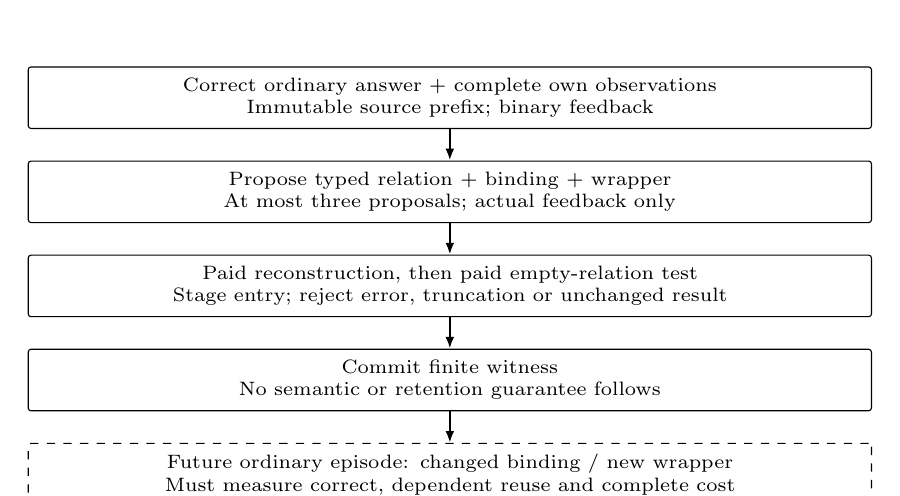
\begin{tikzpicture}[font=\scriptsize,node distance=4mm,
 box/.style={draw,rounded corners=1pt,align=center,text width=0.86\columnwidth,inner sep=4pt},
 edge/.style={-{Latex[length=1.5mm]},thick}]
\node[box] (obs) {Correct ordinary answer + complete own observations\\Immutable source prefix; binary feedback};
\node[box,below=of obs] (proposal) {Propose typed relation + binding + wrapper\\At most three proposals; actual feedback only};
\node[box,below=of proposal] (checks) {Paid reconstruction, then paid empty-relation test\\Stage entry; reject error, truncation or unchanged result};
\node[box,below=of checks] (memory) {Commit finite witness\\No semantic or retention guarantee follows};
\node[box,below=of memory,dashed] (future) {Future ordinary episode: changed binding / new wrapper\\Must measure correct, dependent reuse and complete cost};
\draw[edge] (obs)--(proposal);\draw[edge] (proposal)--(checks);
\draw[edge] (checks)--(memory);\draw[edge] (memory)--(future);
\end{tikzpicture}
\caption{Evidence required at admission and at later use. The dashed box is the
missing empirical milestone. Admission alone is not evidence of useful transfer.}
\label{fig:loop}
\end{figure}

\subsection{Exact-evidence control}
The refined control retains exact complete observations of successful ordinary
SQL executions, even if the episode's final answer is wrong. A failed answer
does not make a valid catalog response false. The final refinement separately
retains every completed episode's submitted answer and Boolean feedback,
including failures. Its initial development configuration retained only
successful-answer receipts; Section~\ref{sec:current} preserves that distinction.
The executable arm receives the same evidence store. A deterministic FIFO cap
of 64\,KiB bounds active evidence and program entries together; duplicate exact
observations refresh their recency. Audit metadata and peak serialized retained
state are reported separately. No model rewrites these observations. Learning checks and other arms'
traces are unavailable. The control therefore directly tests whether retaining
observed conventions and working SQL suffices before adding program discovery.

This control has limits: FIFO can evict a rare but important observation, and
exact results can be stale after drift. Its role is to remove a specific weak
baseline explanation, not to declare text memory solved. Full legal history
remains a separate control, and both retain ordinary direct SQL capability.

\section{Formal guarantees and limits}
The current GH200 audit builds all 90 authored Lean statements, including
89 preserved statements and Proposition~\ref{prop:finite}, with Lean 4.19.0. An
independent imported-environment inventory checks 234 theorem constants,
including generated helpers; 27 authored statements are axiom-free. Other proof
dependencies are confined to the standard axioms \code{propext},
\code{Quot.sound} and \code{Classical.choice}. Six compiler-generated unsafe
runtime specializations are separately inventoried and are not proof premises.
The pinned kernel and standard library remain trusted. These counts describe
verification scope, not novelty. Early manuscripts contained unchecked formal
statements; repaired versions were first kernel-checked in the fifth research
iteration and are checked again here. This does not retroactively verify the
original archived text.

The existing typed-fragment module proves structural substitution and exact
prepared-request preservation for witnessed bindings. It proves explicit CTE
expansion and separation of transported values from SQL text. Giving equal
requests to the same deterministic executor on the same database gives equal
results by equality. This does not formalize SQLite's parser, authorizer,
optimizer or semantics. Python lexical validation and the transport boundary
are checked with executable correspondence fixtures, not a complete refinement
proof.

The preserved guarded-answer theorem returns a supplied ordinary answer after
rejection. Its retention corollary assumes accepted protected answers already
agree with the reference. Runtime fallback instead changes the prompt and
reduces remaining resources; it does not receive a free ordinary answer. The
conditional theorem must not be read as a runtime no-forgetting proof.

\begin{proposition}[Finite dependence does not establish transfer]\label{prop:finite}
For every finite witness set $W\subset\mathbb N$, there exists a candidate that
matches reference answer $1$ on every witness, changes its output when its
relation is removed on every witness, and gives a wrong answer on a fresh
context while still changing under that intervention.
\end{proposition}
\begin{proof}
Let $f_W(x,1)=1$ if $x\in W$ and $2$ otherwise; let $f_W(x,0)=0$.
The second argument represents relation availability. Every witness gives the
correct answer and intervention difference. Choose
$x^*=1+\sum_{x\in W}x$; it is outside $W$, so the candidate's nonintervened
answer is $2\ne1$
and the intervention still gives $0$. The Lean construction uses a finite list
of natural numbers and proves the required fresh element and all equalities.
\end{proof}

The result is an abstract counterexample, not a claim that the model generated
this function or that arbitrary SQL has been verified. It establishes a narrow
logical boundary: any transfer guarantee needs additional restrictions on the
candidate class, observations or evaluation distribution. The proof is not a
sample-complexity lower bound for the implemented learner.

\paragraph{Resource feasibility.}
Let $L$ be acquisition cost, $c_h$ a competent direct-query cost, and
$c_m=g+e$ the checked-use cost of a guard plus execution. Reusing a candidate
$n$ times saves SELECTs only if
\begin{equation}\label{eq:amortization}
 L+n c_m<n c_h.
\end{equation}
If $c_h=1$, $g\geq1$ and $e\geq1$, this is impossible for $L\geq0$ and $n>0$.
When $c_h>c_m$, the break-even requirement is $n>L/(c_h-c_m)$. This accounting
observation is not a general lower bound on all memory systems: a different
validator or task can have different costs. It does rule out SELECT savings
for the present path against a one-query baseline. Token and latency gains
remain distinct, measurable hypotheses.

\section{Preserved empirical evidence}
The historical tables distinguish synthetic controlled evaluations from adaptive
language-model development. All language-model results below are development
evidence. Adaptive diagnostics
and independent follow-ups are kept separate. A replay verifies consistency
with recorded SQL, prompts, transitions, source freezes and costs; it does not
independently authenticate model weights or backend token counts.

\subsection{Controlled learning before the language-agent study}\label{sec:historical}
The earlier experiments isolate capabilities that are otherwise confounded in
an end-to-end agent: exact evidence reuse, recurrence recovery, neural
interference, exploration choice and statistical opportunity cost. Their
synthetic reward scales and feedback differ, so their scores are not pooled
with SQL accuracy or normalized into a common leaderboard. Tables below report
saved results; no historical model or learner was rerun for this consolidation.

\paragraph{Compression preserves both competence and failure.}
The initial fixed-class symbolic study compares witnesses with full replay over
20 seeds and 384 episodes on four public arithmetic scopes. On the interleaved
scenario both achieve 94.17\% whole-stream and 100\% late reward; witnesses
use 2340.9 mean hypothesis evaluations versus 78,146.15 for replay, with 29.4
active constraints. These are symbolic-operation savings, not measured model
tokens or inference latency. Both learners also fall to 15.91\% late reward
under hidden shifts and 14.09\% under misspecification, producing four wrong
certificates per seed in each case. Compression preserves a fixed inference
rule, including its failures when coverage or stationarity is false.

\paragraph{Recurrence recovery.}
Twenty-seed arithmetic microstudies compare the original fixed-class learner,
epoch resets, and resets with archive-weighted recovery. Stationary and fresh-
input late accuracy reaches 100\% in all three, demonstrating finite-class
learning under exact feedback. Under recurring rules, archive reuse reaches
97.70\% late accuracy versus 84.02\% for resetting alone. Under rapid switches,
those scores fall to 22.48\% and 17.60\%; under noisy feedback they are 65.18\%
and 47.62\%. These stress failures violate the clean fixed-epoch assumptions
needed by the exact elimination argument.

Typed relational plans show the same boundary: recurring-recipe late accuracy
is 97.45\% with archive reuse versus 63.59\% with resets alone, but the
out-of-grammar multiplication diagnostic stays below 0.11\% across controls.
Supported sum/difference expressions transfer to fresh rows; grammar support
and semantic discovery are not interchangeable. The arithmetic and relational
summaries contain both whole-stream and late accuracy; the figures here are
explicitly the latter. None is a native language-agent benchmark result.

\paragraph{Admission opportunity cost.}
A separate live randomized one-step auditor, using only its chosen action's
outcome, reaches whole-stream reward .8905 on the stationary task versus .9437
for its ungated proposer, and .7544 versus .8692 under recurrence. Both stationary
late scores reach one. The auditor's useful protection and eventual learning do
not repay its transient exploration and delay on these twenty-seed studies.
This is an early instance of the cost problem later exposed more sharply in the
SELECT-budget comparison.

\paragraph{Parameter learning.}
In 24-dimensional fixed-feature residual experiments, rank-four protection
reduces new-task MSE from 25.070 to 4.226, with mean maximum protected drift
$2.02\times10^{-16}$. Rank-twelve protection leaves MSE 12.958; full-rank
protection leaves the original 25.070 unchanged. Twenty seeds per rank quantify
both trainability and the capacity cost predicted by Eq.~\eqref{eq:residual}.
This is floating-point linear residual learning, not an empirical theorem about
LLM weights.

\begin{table}[t]
\centering\small\setlength{\tabcolsep}{4pt}
\begin{tabular}{lrrr}
\toprule
Neural update & Late acc. & Forgetting & Updates\\
\midrule
Shared, width 24 & 96.13\% & 47.09 pp & 4800\\
Shared, width 72 & 96.26\% & 44.58 pp & 4800\\
Shared + replay & 96.23\% & 2.65 pp & 9599\\
Three frozen modules & 95.43\% & 0.00 pp & 4800\\
\bottomrule
\end{tabular}
\caption{Separate online neural diagnostic over 20 seeds and three public
scopes. Late accuracy averages the last 200 of 1600 interactions per scope.
Forgetting averages acquired-minus-later held-out accuracy across old-scope
checkpoints. Fixed routing
makes the frozen-module result structural. These are not language-model
fine-tuning results.}\label{tab:neural}
\end{table}

Table~\ref{tab:neural} compares learned feature modules with shared networks.
The three frozen width-24 modules use 4056 parameter bytes, near the shared
width-72 model's 4040 bytes, and show zero measured old-logit drift. Replay uses
an additional 10,752 replay payload bytes, excluding Python overhead, and about
twice as many updates. Its late
accuracy is slightly higher than isolation. All methods receive authentic
public scope information; module storage grows as scopes are added. The
384,000 interactions are 20 seed replications across four arms, not 384,000
independent trials. Each scope has 512 fixed fresh test inputs. The historical
artifact preserves per-seed summaries rather than complete interaction traces,
limiting retrospective diagnosis of individual training events.

\subsection{Information value and the cost of exact planning}
The earlier supplied-model controller runs 17,920 episodes over 20 seeds, two
finite-world domains and seven arms. With exploration budget $B=4$, it exactly
ties full-history optimistic planning in late return, averaged over the final
16 of 64 episodes, on every seed in both domains. On delayed damage, mean late return is 13.1375; requiring $B=0$ reduces
it to 12.5625. The immediate-reward greedy control reaches a worst cumulative
anchor deficit of 133, compared with two for $B=4$ and zero for $B=0$. These
are native simulator returns and deficits, not accuracy or an ICL comparison.
The experiment illustrates conditional exploration protection and its cost,
without establishing a reward advantage over history planning.

The finite-transducer controller with a trainable proposer improves by only
.0142 reward per episode over its no-training ablation at budget $B=64$.
Informative probing improves by .0567 over unguided probing. Neither comparison
establishes superiority to a strong planner: at $B=16$, the controller trails
full-history symbolic planning by .03708, with paired 95\% interval
$[-.05528,-.01888]$, while late return on the returning objective ties. This
full-history planner is symbolic inference, not LLM ICL.

A proposed one-probe minimax-regret objective then failed its frozen test:
mean reward fell .09458 relative to the earlier controller, interval
$[-.16915,-.02001]$, while measured mechanics time was about $1.90\times$ larger.
A post-hoc weak-dominance repair improved ten of the 256 enumerated tables
without worsening one relative to that failed rule, but remained below stronger
controls. The correction is a separate diagnostic, not a replacement holdout.

The reason one-step information value can fail is concrete. Suppose two free
probes reveal bits $a,b$ and the valuable action depends on $a\oplus b$.
Neither individual bit changes the immediate minimax regret, yet both together
identify a better zero-loss decision. Requiring positive one-probe regret
reduction stalls forever. Depth-two planning resolves this construction, but
an analogous three-bit parity defeats it. The cheap rule that accepts any
informative zero-loss probe reaches the correct decision after three probes.
A deeper fixed horizon shifts this failure without establishing exploration
completeness.

\begin{table}[t]
\centering\small\setlength{\tabcolsep}{4pt}
\begin{tabular}{lrrr}
\toprule
Finite-class selector & Reward & Plan sec. & Spent risk\\
\midrule
Depth two & 4.19688 & 8.3439 & 1.775\\
Informative zero-loss & 3.80313 & .9398 & .000\\
Bounded optimism & 4.39167 & 1.5603 & 6.975\\
\bottomrule
\end{tabular}
\caption{Forty-stream finite-class evaluation with shared work/deadline rules
and $B=16$. Equal budget ceilings do not imply equal realized risk or time.
Reward is this simulator's return per episode, not accuracy.}\label{tab:planning}
\end{table}

On the forty-stream comparison in Table~\ref{tab:planning}, depth two beats the
zero-loss rule by .39375, paired interval $[.15845,.62905]$, but takes
$8.878\times$ its planning time. It loses .19479 to bounded optimism, interval
$[-.31761,-.07198]$. Only the former was primary; the other comparisons are
exploratory and unadjusted for multiplicity. A cooperative search cap produces
\code{UNKNOWN} on 30.73\% of depth-two decisions. Smaller computation ceilings
remove its primary reward gain. Exact checking remains authoritative, so these
failures concern useful search and cost rather than a detected ledger violation.

A separate five-world local-LLM smoke study executes 120 model calls. The first
world has no action-dependent headroom and all arms score 5.3333. On four
exploratory extension worlds, the checked hybrid scores 5.5417 versus 3.9583
for raw model history and 5.0000 for a fixed-library checked control. The hybrid
also has finite-model inference and an online proposer; the fixed-library
control still trains that proposer. Five worlds and unequal machinery cannot
establish memory superiority or model-weight learning.

\subsection{Feature reuse works within a grammar, then loses its budget}
The sixteen-stream relational study contains a prospectively specified positive
result: prioritizing previously promoted nonlinear features improves reward on
the first 24 shared-novel encounters by .12240 over the otherwise matched
no-reuse grower, paired 95\% interval $[.03158,.21321]$. The first-eight contrast
is exactly zero. The result supports later feature-search transfer within the
supplied grammar; it does not show immediate or unconstrained discovery.

\begin{table*}[t]
\centering\small
\begin{tabular}{lrrrrrr}
\toprule
& \multicolumn{3}{c}{Equal ordinary-example schedule} &
\multicolumn{3}{c}{Common 4096-SELECT ceiling}\\
\cmidrule(lr){2-4}\cmidrule(lr){5-7}
Method & Shared first 24 & Final macro & SELECTs & Final macro & Examples & Audit pairs\\
\midrule
Growing + reuse, audited & .1745 & .6807 & 4889.9 & .4744 & 138.1 & 582.6\\
Growing, no reuse, audited & .0521 & .7344 & 4939.3 & .4744 & 139.8 & 581.6\\
Sparse history, audited & .5130 & 1.0000 & 2440.9 & 1.0000 & 903.6 & 123.2\\
Sparse history, ungated & .5469 & 1.0000 & 1824.0 & 1.0000 & 1109.0 & .0\\
Full ridge, ungated & .0026 & .0000 & 1824.0 & 1.0000 & 1109.0 & .0\\
Growing all 84, audited & .0729 & .7876 & 4981.2 & .5117 & 136.6 & 583.4\\
\bottomrule
\end{tabular}
\caption{Saved relational evaluation, sixteen independent seeds per protocol.
Entries are mean arm/run outcomes. The matched schedule gives every arm 224
ordinary examples; the budget schedule exposes the audit's opportunity cost.
SELECTs exclude database setup, whose time is accounted separately.}\label{tab:relational}
\end{table*}

Table~\ref{tab:relational} shows why this positive ablation is insufficient.
Under the same 4096 post-setup SELECT ceiling, reuse attains .4744 final macro
reward versus 1.0000 for all three fixed simple controls: audited sparse
history, ungated sparse history and ungated full ridge. The paired difference
is $-.52563$, interval $[-.55610,-.49517]$. Auditing consumes queries that those
controls spend on ordinary learning. Ordinary execution costs three SELECTs
(two measurements and one feedback query); paired audits cost five. Database
creation is outside that named query budget, and wall time is not equalized.

At the end of matched training, only 34.4\% of shared-novel reports contain all
true terms in the selected feature set; 71.9\% reach the width cap. These are
evaluator-only diagnostics on saved policies, not learning hints. Old-report
policies and predictions do not change during novel learning because report
dispatch is authentic and frozen. That structural retention is real within its
contract, but it does not test learned routing, hidden drift or shared neural
parameter retention.

The full evaluation contains 192 arm/runs, 78,081 ordinary episodes, 61,790
paired audits and 61,440 panel contexts, with 727,513 post-setup SELECTs.
Independent seeds, rather than those correlated episode counts, support the
reported intervals. A point estimate above .05 with an interval above zero
supports positive mean gain; it does not certify gain exceeding .05.

\paragraph{Historical evaluation boundaries.}
Fresh random seeds were not always new worlds. The 100-seed transducer
comparison sampled 81 unique worlds, six overlapping development. The later
one-probe study had 85 unique evaluation worlds and ten shared with its pilot.
These are within-family evaluations, not disjoint-world generalization. A
post-evaluation backend/DAG optimization preserved all selected behavior fields
across 38,400 earlier rows but changed timings; timing results must retain their
execution provenance. The forty-stream depth-two evaluation happened to have
zero overlap with its eight development worlds, although sampling allowed
replacement. Initial development preceding independently found implementation
corrections remains in the archive and is excluded from the final-protocol
replay count. No corrected or post-hoc result is relabeled as an untouched
holdout.

\subsection{A failed prerequisite in the language-agent pilot}
The v8 configuration used Qwen3-4B Q8\_0 across six arms: full history, retrieved
episodes, evolving insights, checked and unchecked fragments, and stateless
solving. Every arm scored 0/8 on the warm block. All 288 scheduled arm-episodes
completed; neither fragment arm admitted a program or performed a
\code{USE}/\code{COMPOSE} action. Every old-task answer before and after was
wrong. The 14 correct answers elsewhere in the schedule were all zero.

The pilot spent 307 SELECTs, including 141 SQL errors, and 621 model calls
containing 1,138,451 reported tokens in 690.13 seconds. A lower query count for
an unsuccessful arm is not a learning advantage. These results apply to that
configuration, not to the feasibility of executable memory in general.

\subsection{Competence improves, but memory does not yet transfer}
Seven adaptive v9 diagnostics on one development seed tested interface
instructions, decoding and model choice. Four 4B variants scored 0/8. Two
nonthinking Qwen3.5-9B Q8\_0 variants scored 1/8 and 0/8, while a thinking
configuration with explicit live-tool interaction reached 7/8. Several factors
changed; this is not an isolated causal estimate of reasoning or model size.

Three separately frozen follow-ups used fresh development seeds. The first
stopped at native schema generation; the second was intentionally stopped after
malformed memory responses and a forced reasoning cutoff. The final adapter
retained host validation while repairing native schema compatibility and
reasoning handling. Table~\ref{tab:warm} records its entire completed warm block.

\begin{table}[t]
\centering\small\setlength{\tabcolsep}{4pt}
\begin{tabular}{lrrrr}
\toprule
Method & Correct & SELECTs & Calls & Tokens\\
\midrule
Full history & 8/8 & 9 & 17 & 50,178\\
Evolving text & 6/8 & 14 & 30 & 55,808\\
Checked programs & 7/8 & 22 & 31 & 49,700\\
\bottomrule
\end{tabular}
\caption{Final v9 development warm block, seed 92003. Every arm started empty
with the same solver and episode allowance. Unequal accuracies prevent a
matched-accuracy efficiency interpretation. Exact evidence is a later control
and has no result in this table.}\label{tab:warm}
\end{table}

The predeclared rule required every arm to reach at least 7/8. Text memory
failed, so only 24 of 144 planned records ran. Old-task, transfer and final
composition panels did not execute. Checked programs made seven proposals and
two finite admissions, with zero later \code{USE}/\code{COMPOSE} actions.
Its 7/8 measures ordinary solving, not executable transfer.

All seven diagnostics and three follow-ups comprise 89 records and 244
requests: 366,795 known tokens, two failures with unknown actual usage, and
1104.03 measured seconds. Declared reservations for the failed calls give an
upper total of 375,904 tokens; this is a bound rather than an observed exact
total. Setup and download are separate. These timings are historical and are
not GH200 throughput measurements.

\subsection{Two admitted programs, two different weaknesses}
One admitted program computes a refunded-order scalar. Emptying it changes its
wrapper result from 22 to NULL. However, the generator makes the count 22 by
construction, and its integer parameter merely turns rows on or off. No
changed-binding transfer occurred. A dependent scalar template is weaker than
a reusable row-level abstraction.

The second program computes a Gold-tier total. Its wrapper repeats the
physical-table query and ignores the learned relation. Emptying, removing,
replacing or rebinding the relation leaves 1350.25 unchanged. The stored program
itself returns the observed answer; the defect is that its admission witness
does not establish its contribution. Eleven offline SQL probes on saved
fixtures establish this mechanism result. They supply no learner observations
and change no recorded scores or costs.

The text failures are also specific. One summary omitted the documented
NULL-as-zero averaging convention; a later query used ordinary AVG and dropped
NULL rows. Another memory state omitted units, quantities and exact join keys;
the subsequent query joined incompatible identifiers and summed raw units.
These observations motivate exact evidence preservation. No paired intervention
isolates compression as the sole cause: the solver could have reread the catalog.

\subsection{Status of the current refinement}\label{sec:current}
The GH200 runner compares full history, exact evidence and repaired programs,
each starting empty. Eight warm questions precede an eight-item frozen old
panel, 16 further ordinary questions, the same old panel, and eight final
questions: 48 episodes per arm, 144 planned records per study. Every arm must
score at least 7/8 warm before proceeding; frozen panels cannot update memory.
These are new development studies, not native benchmark evaluations.

The runtime uses official Qwen3-32B Q8\_0 weights, a pinned CUDA llama.cpp build
and one GH200 with approximately 96 GiB of device memory. The 65,536-token
context uses explicit YaRN extension beyond the native 32,768 positions. Source,
model and runtime inventories are bound before each study. Solving enables
thinking with temperature .6, top-$p$ .95, top-$k$ 20, minimum probability zero,
presence penalty 1.5 and sampling seed 42. Solve and nonthinking proposal calls
allow at most 2048 and 4096 generated tokens. Setup and a generic transport smoke
check are separate from study cost. Changed model and runtime prevent a causal
cross-version attribution to memory alone.

\begin{table*}[t]
\centering\small\setlength{\tabcolsep}{3pt}
\begin{tabular}{llrrrrrr}
\toprule
Stream & Method & Episodes & Warm & All SELECTs & All calls & Known tokens & Admitted\\
\midrule
94000 & Full history & 8 & 7/8 & 13 & 21 & 78,033 & 0\\
94000 & Exact evidence & 8 & 4/8 & 9 & 17 & 39,567 & 0\\
94000 & Checked programs & 8 & 4/8 & 17 & 23 & 49,424 & 2\\
94001 & Full history & 22 & 8/8 & 34 & 56 & 342,897 & 0\\
94001 & Exact evidence & 22 & 7/8 & 25 & 48 & 190,543 & 0\\
94001 & Checked programs & 22 & 7/8 & 51 & 70 & 247,317 & 5\\
\bottomrule
\end{tabular}
\par\smallskip{\footnotesize Costs cover all recorded phases; the Warm column covers only the first eight ordinary questions. Known tokens exclude unmeasured usage.}

\caption{GH200 development receipts. These adaptive studies are separate
configurations. Counts include failures, checks and the final interrupted
follow-up episode; only 65 of its 66 saved records complete. The program arm's
follow-up tokens exclude one call with unknown usage. Lower costs at unequal
accuracy do not establish matched-accuracy efficiency.}
\label{tab:gh200cost}
\end{table*}

\paragraph{Initial development.}
Stream 94000 completes 24 warm records and fails the all-arm gate: full history
scores 7/8, exact evidence 4/8 and programs 4/8. All initially use integer
division for currency despite the catalog's real-arithmetic convention. History
later corrects it. The evidence shelf retains successful SQL executions but
omits failed-answer receipts, withholding a useful failure signal. This is a
weakness of that configuration, not a general failure of exact memory. Two
programs pass reconstruction and dependence; neither is subsequently executed.
The run uses 61 calls, 167,024 tokens and 577.38 study seconds, with no unknown
usage. Transfer and retention remain untested after the gate stops it.

\paragraph{Final adaptive follow-up.}
A separate freeze precedes seed 94001. The shelf now retains every completed
answer and Boolean feedback, and every arm receives the same generic SQLite
integer-division instruction. No hidden target or domain query is supplied.
Both changes are selected after the first failure, so this is not a causal
ablation or heldout evidence. All warm scores meet the threshold and the runner proceeds.\footnote{The final
manifest's \code{warm\_qualified} flag remains false because it additionally
requires a completed study; the warm-score threshold itself passed.} The fresh
old-panel scores are 6/8, 2/8 and 4/8 for history, evidence and programs.
Table~\ref{tab:gh200phase} keeps the later comparison to common finished
questions. Figure~\ref{fig:gh200warm} shows qualification, not a transfer curve.

\begin{table}[t]
\centering\small\setlength{\tabcolsep}{3pt}
\begin{tabular}{lrrr}
\toprule
Method & Warm & Old before & Later shared\\
\midrule
Full history & 8/8 & 6/8 & 4/5\\
Exact evidence & 7/8 & 2/8 & 4/5\\
Checked programs & 7/8 & 4/8 & 3/5\\
\bottomrule
\end{tabular}
\caption{Follow-up accuracy on completed matched questions. Later shared is
ordinary indices 8--12, only five of the planned sixteen later questions.
Index 13 is correct for history and evidence but interrupted for programs,
so is excluded here and included in total costs. Failed completed attempts
count as zero. Old-after and final panels have no observations.}
\label{tab:gh200phase}
\end{table}

\begin{figure*}[t]
\centering
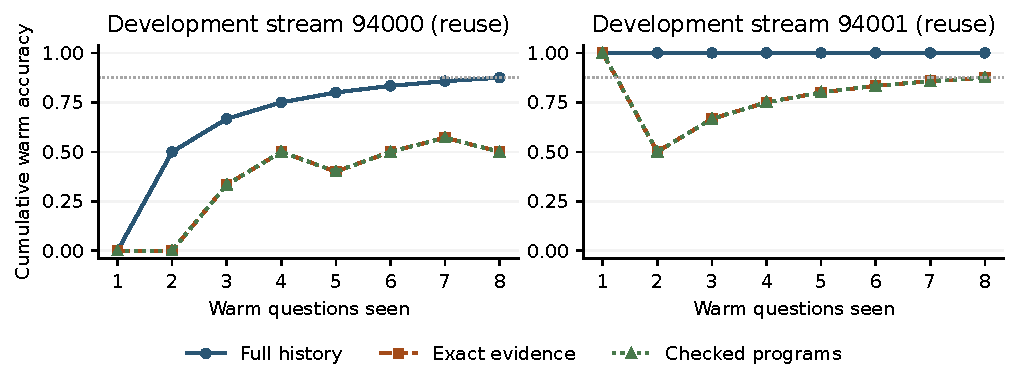
\includegraphics[width=.92\textwidth]{gh200_warm.pdf}
\caption{Cumulative accuracy over the eight warm questions in each adaptive
development stream. The horizontal line marks the final qualification threshold,
not a requirement at every prefix. These curves establish neither stateful gain
against reset memory nor transfer to fresh instances.}
\label{fig:gh200warm}
\end{figure*}

The follow-up stops at its deadline with 66 saved records out of 144 planned,
including one interrupted program-arm episode; 65 records complete. It uses
174 generation attempts and 780,757 known tokens. The interrupted call has
unknown usage, so the token total is incomplete and the receipt does not mark
usage verified. Recorded time is 2700.024 seconds: incremental export exceeds
the 2700-second ceiling by .024 seconds, and the receipt marks that cap
unsatisfied. Neither later old-panel nor final-panel evaluation occurs. Five
relations are admitted, but none executes through the checked \code{USE}/\code{COMPOSE}
path on a future question.
The intended execution mechanism is not demonstrated, and retention is
unassessed; missing panels are not zero-regression evidence.

Across both studies, resource expenditure is 235 calls, 947,781 known tokens
plus one unmeasured call, and 3277.40 study seconds. Accuracy is not pooled
across these adaptively changed configurations. The aggregate allowance is
3600 seconds, 4M tokens and 1800 attempts; exact compliance with the token
allowance is not asserted with missing usage. No further model-task attempt is
made in this phase, and reserved heldout seeds remain unused. Source hashes are
unchanged. Source-bound replay verifies 65 complete follow-up traces and 110
recorded SQL executions, separately identifying the partial trace. This is a
partial-study audit, not completion of the experimental protocol.

\paragraph{What the repair actually changes.}
On the follow-up total-refunds task, the first wrapper repeats a physical-table
subquery and aliases it as \code{reused}, shadowing the learned CTE.
Reconstruction returns 2311.75, but emptying the learned relation still returns
2311.75, so admission is rejected. The next proposal reads the actual
\code{reused} relation: reconstruction remains 2311.75 and the intervention
returns zero. It is admitted after four charged check SELECTs plus the ordinary
query. This is model-driven defect repair on one candidate, not later transfer.

Applicability is a distinct failure. The North-customer relation stores a guard
requiring the old customer count, six. A later proposed composition observes
three; a frozen old-panel count question observes four. Both guards reject
before the relation executes. The old-panel episode nevertheless answers
correctly with the guard's fresh count as its only current SQL result. This
records useful source-query reuse, without a counterfactual establishing the
answer's causal dependence on that result. Zero proposed-relation executions
therefore does not mean zero memory influence. The attempted composition also
contains an unsupported substitution placeholder; its validity is unestablished.

Finally, the old panel exposes stale scalar replay. History, evidence and
programs answer without SQL on two, six and four questions respectively; zero,
one and one of those answers are correct. The interface changes rows without
exposing a snapshot identifier, while reusing question text and schema. This
makes freshness an interface as well as a memory issue. Exact retained results
and a successful warm gate do not ensure fresh-instance competence, and no
paired intervention here isolates one cause of these failures.


\section{Falsifiable next mechanisms}
\subsection{Ground the answer in a current execution}
The interface should first make observation freshness explicit: the fixture
can change rows while reusing a question and schema, without exposing a database
snapshot identifier. A cheap prospective control supplies that identifier and
a generic statement that earlier scalar results may be stale. This changes no
hidden target or convention. It must be compared separately with the stronger
intervention below, because stale answers need not be a memory-only failure.

A separate proposed repair makes the answer action refer to a complete numeric
result from a query executed in the current episode. The host resolves the
receipt and emits the stored value; the model cannot supply a replacement
number or a receipt from a previous episode. This would apply equally to every
arm, including full history, and its query costs remain charged. It targets
stale scalar replay rather than reusable representation learning.

The operational hypothesis is that current execution receipts reduce wrong
answers copied from previous fixtures at useful total cost. Test the interface
change on independently selected development streams, compare with an identical
free-number answer interface, and preserve every error and added query. Kill
its practical claim if accuracy does not improve enough to repay those costs.
A constant query can still reproduce an old scalar; requiring a physical-table
read would close only the simplest loophole. Neither a read nor a current
receipt establishes that the query answers the question. This is an
unimplemented experiment, not a theorem of semantic correctness.

\subsection{Corroborate a relation before promoting reuse}
\paragraph{Hypothesis.}
A useful executable memory should preserve a relation that supports multiple
future operations, while text retains the exact evidence needed to interpret
it. We propose keeping a relation provisional until an independently encountered
future episode corroborates it with a meaningful changed binding. This is an
unimplemented extension beyond the bounded repair, not an empirical result.

The learner first proposes a row-level relation from a correct own query,
retaining its output columns and source computation. Admission continues to
require charged reconstruction and dependence. A restricted outer language
would read only the supplied learned relation, literals and approved pure
operations; physical table access remains in the inner program. Enforcing that
restriction requires a real SQL semantic-access boundary, not substring checks.
It prevents the specific independent recomputation, but cannot certify intent.

A useful admission ablation would apply a supported-fragment equivalence checker
to the complete source and reconstruction, using no hidden target query.
Bounded counterexamples should be replayed in SQLite to detect dialect or
semantic-model mismatches. Record proof, counterexample and unknown separately;
an unsupported feature or timeout is not an admission. A CPU solver budget is
charged alongside model cost. Kill this addition if supported coverage is too
small, counterexamples fail to reproduce, or checking cost erases useful later
gains. Even an unbounded source-equivalence proof would protect only that
source computation, leaving intended semantics and new operations unproved.

Applicability needs its own repair. Current guards can require an old aggregate
to remain exactly unchanged. That can reject a valid relation after rows change,
while an unchanged aggregate can conceal a convention change. A prospective
ablation would instead compare exact observed schema and catalog conventions,
leaving variable data out of the compatibility key. This uses learner-visible
metadata, not evaluator scope identifiers, and its reads are charged. It still
requires truthful documentation and cannot validate a bad inferred relation.

A provisional relation is not counted as useful learning. Freeze its code and
source wrapper. When a later ordinary question naturally makes the same source
operation relevant, the solver first answers without using this candidate. After
correct feedback, the agent may spend its remaining allowance on reconstruction
with a proposed new binding, comparing it with the new own successful query.
These observed answers must agree, and both the binding and observed
nondegenerate output must differ from the original witness. The learner receives
only its ordinary observations and binary feedback; the evaluator does not
schedule a hidden task identifier as a retrieval hint. A separate later question
must use a new outer operation on fresh rows and depend on the stored relation.
The evaluator audits provenance, actual parameter changes, output variation and
correctness after the learner has finished.

This design separates three milestones: a checked proposal, a corroborated
source computation, and useful new composition. It can still fail. Two samples
need not identify the intended relation; a misleading proxy can pass; a valid
relation may never recur; and extra corroboration may erase every future cost
saving. The outer restriction can exclude useful joins. These are reasons to
run the following experiment before adding a more elaborate architecture.

\subsection{Experiment and decision rules}
Freeze model revision, effective decoding, prompts, all update rules,
retrieval/cap policies, generator, seeds and resource ceilings before each new
study. Reserve separate development and confirmatory streams, including fresh
numeric data and semantic conventions where the generator supports them.
Never pool the earlier adaptive diagnostics as independent replications.

The current three-arm development comparison uses full history, exact evidence
and repaired executable memory. All start empty. Every arm must first pass the
same competence gate. The mechanism extension then requires a separate freeze
and at least the following comparisons: no persistent memory, full history,
exact evidence with SQL, bounded repair, and delayed corroboration. A faithful
published evolving-text method is needed before claiming an advantage over
modern memory systems. An ablation giving the same extra direct queries to the
control distinguishes representation benefits from additional evidence.

Use shared-reuse, nonreuse and near-match/drift streams. Measure old panels on
fresh instances before and after learning with updates disabled; evaluate
changed binding and new outer operation separately. Complete schedules are the
unit of replication. Report each stream's accuracy, stateful gain, query cost,
input/output tokens, latency and retained bytes, including rejected proposals
and checks. Do not analyze correlated episodes as independent streams.

\paragraph{Chosen useful effect, not an established threshold.}
A reasonable next target is at least five percentage points of future accuracy
improvement over the best qualified compact control, no more than two points
of loss against the protected reference on old-scope accuracy, and a 20\%
token reduction against full history at qualified accuracy. These are separate
endpoints: passing one does not compensate for failing another. They require
prospective finalization after development establishes achievable accuracy and
variance, before confirmatory evidence is seen. SELECT savings should be
abandoned on cases subject to Eq.~\eqref{eq:amortization}, rather than hidden
inside another metric.

Kill the mechanism as a practical improvement if exact evidence matches its
accuracy at lower total cost, if apparent transfer disappears after source or
binding interventions, or if it rarely produces a later correct composition through the intended execution
route. Zero checked relation executions would not show that visible program
text or stored guard queries had no effect on the solver.
Reject a retention claim whenever its predeclared noninferiority test fails;
an underpowered interval is inconclusive, not proof of preservation. Any
future-label leakage, uncharged repair or mutable frozen panel invalidates the
comparison even if its score is high. A negative result should terminate the
corresponding claim rather than trigger repeated evaluation on the same seeds.

\subsection{Resources and statistical feasibility}
The current GH200 supports the selected 32B inference runtime, alongside CPU
SQLite execution and local artifact storage. A query-equivalence ablation would
add a CPU SMT solver; online weight adaptation would additionally need optimizer
state and update compute. These are distinct resource requirements.

A three-stream, three-arm, 48-episode-per-arm pilot has 432 planned records.
Warm-question cost is an unreliable estimate of its full cost: later questions
in the current study require several minutes of reasoning and repeated failed
queries. There is no validated complete-schedule runtime estimate. A bounded
future pilot could allocate at most one GH200-hour, one million tokens and
600 generation attempts per arm and stream: nine accelerator-hours, nine million
tokens and 5400 attempts in total, with setup separate. These are proposed
ceilings, not a promise of schedule completion. Additional causal ablations
require additional arms and budgets. Reserve resources for frozen evaluation
before allocating discovery work; missing required panels leave retention
unassessed. Development must establish completion and useful transfer within
the ceilings before a larger confirmatory commitment.

For a broader comparison, determine independent-stream count from development
variance and the fixed endpoints. As a planning approximation for a paired mean
difference, $n\approx(z_{1-\alpha}+z_{1-\beta})^2\sigma_D^2/\delta^2$;
account for all endpoints and use conservative variance estimates. For example,
with $\sigma_D=0.10$, 80\% power and a one-sided 0.005 endpoint level, detecting
$\delta=0.05$ needs about 47 streams, whereas resolving a 0.02 retention margin
needs about 292. These normal approximations are not guarantees, and clustered
or nonstationary data require a justified model. A short development run cannot
support a two-point no-forgetting headline.

For perspective, even observing no regression in 32 independent Bernoulli
trials only bounds the event probability by about 8.9\% with a one-sided 95\%
exact interval. Episodes sharing a stream do not automatically supply 32 such
trials. Retention is a substantial experimental requirement, not an adjective
attached to an immutable library.

\section{Training, inference and deployment boundaries}
The present SQL language agent changes external state during deployment. Its training
signal is its own permitted observations, execution errors and binary task
feedback. It performs no offline model retraining and no online gradient
updates. This isolates the representation experiment, but it may leave the
solver unable to discover useful relations even with a sound admission rule.
Increasing model capacity can address competence; it cannot retrospectively
turn ordinary SQL into learned reuse.

A later online LLM adapter is a distinct proposal: train only on independently
verified own successful traces, keep an immutable reference model, and test
candidate updates on fresh protected tasks before promotion. It would need
optimizer state, replay/storage accounting, update compute, and a full-history
control using the same examples. No such adapter or retention result is claimed
here. Offline meta-training for updateability also changes the resource and
supervision comparison.

During inference, rejected guards consume budget and can influence subsequent
reasoning. A deployment requiring a hard service fallback must reserve enough
resources for the reference path and specify its inputs and environment state.
Merely retaining a reference checkpoint supplies none of those conditions.
Observations and generated memory are data, not authority to modify the executor.
Database read-only enforcement and deterministic source provenance reduce
specific implementation risks; safe decision-making beyond those boundaries
remains a separate task.

\section{Limitations and research value}
The strongest general comparison remains negative. The current fixture has a
small set of conventions, a revealing catalog and one structurally constant
target. The v8 solver was inadequate, and the competent v9 follow-up stopped
before transfer. The v9 interventions diagnose two saved programs, not a
population of learned abstractions. New GH200 traces separately demonstrate
repaired admissions, stale answers and guard failures. The exact-evidence
control and repair address observed defects; they do not establish a general
solution. The final GH200 study exceeds its wall ceiling by .024 seconds during
export, has one call with unknown token usage, and lacks its later retention
and final panels. None of these gaps is silently filled by a model or estimate.

The potentially useful result is a more demanding unit of evidence. A memory
entry should not count as acquired competence until its computation contributes
to a correct later task under meaningful variation and complete resource
accounting. Even then, retention and benchmark superiority require separate
measurement. A strong future paper must demonstrate that conjunction against
competent full history and modern memory controls on independent stateful
streams. The next decisive evidence is correct dependent reuse on completed controlled
streams, followed by a qualified retention comparison.

\appendix
\section{Recurrence, noise and limited storage}\label{app:recurrence}
\subsection{A recurrence-sensitive mistake bound}
Within one deterministic, realizable, unchanging inference epoch, assign each
rule $h$ positive prior mass $\pi(h)$. Predict a maximum-mass action and delete
rules contradicted by the exact chosen-action feedback. If at most $K\geq2$
distinct actions are predicted, a mistake removes at least $1/K$ of surviving
mass. The true rule keeps its original mass, so after $M$ mistakes
\begin{equation}
 \pi(h^*)\leq(1-1/K)^M,\qquad
 M\leq\frac{\log(1/\pi(h^*))}{-\log(1-1/K)}.
\end{equation}
This is the standard weighted-elimination argument specialized to recurrence.
If an archive $\mathcal A\subseteq\mathcal H$ receives prior mass $\beta$,
\begin{equation}
 \pi(h)=\frac{1-\beta}{|\mathcal H|}
       +\frac{\beta}{|\mathcal A|}\ind\{h\in\mathcal A\},
\end{equation}
a returning archived truth has $\pi(h^*)\geq\beta/|\mathcal A|$ and therefore a
smaller recovery bound than a uniform new search when the archive is useful.
An empty archive uses the uniform prior. The reference uses $\beta=4/5$.

Contradiction first triggers bounded grammar growth with complete evidence
backfill; if no consistent interpretation remains, an internal epoch restarts
while old programs stay archived. The epoch is not a supplied hidden regime
identifier. A uniquely identified rule in a fixed class encounters a
contradiction on its first wrong post-change prediction, but the argument does
not cover a still-ambiguous class, noise, rapid switches or a newly constructed
mixed-history explanation. The stress failures reported in the main text are
therefore substantive limits, not violations of the clean-epoch theorem.

\subsection{Noise needs probabilistic evidence, not harder deletion}
A separate component assumes a fixed finite collection of proper conditional
outcome models that includes the true model. Fix weights $\pi_m>0$ with
$\sum_m\pi_m=1$ before observing data,
let $L_{m,n}$ be model $m$'s likelihood of the actual chosen-action outcomes,
and define
\begin{equation}
 E_{m,n}=\frac{\sum_j\pi_jL_{j,n}}{L_{m,n}}.
\end{equation}
On paths with positive true-model likelihood, likelihood ratios are nonnegative
supermartingales under that model, and martingales with appropriate common
support. Predictable adaptive actions do not break the conditional likelihood
argument. Consequently, excluding $m$ only after
$E_{m,n}\geq1/\delta$ retains the actual fixed model at all times with
probability at least $1-\delta$.

The implementation uses exact rational arithmetic in small examples and checks
all binary histories of length six for a common-support example. In 1000
independent 64-step diagnostics with 10\% noise and nominal $\delta=.05$, the
probabilistic filter ever excludes truth in 12 sequences, versus 997 for hard
deletion. This finite simulation illustrates the distinction; it is not a proof
of the nominal coverage probability. This is a
separate tested statistical component, not a stochastic extension of the
integrated deterministic controller or a Lean proof of probability theory.
Uncalibrated neural scores are not specified conditional probabilities. Models
chosen after seeing old data cannot receive retroactive likelihood credit, and
stochastic realized returns need their own deviation argument beyond the
pathwise deterministic debit bound.

Soft fixed-archive routing is also implemented separately through importance-
weighted feedback and fixed-share expert updates. It keeps alternatives alive
when hard deletion is inappropriate, but provides an expected tracking bound
rather than per-episode protection. For rapid switches, the stated regret bound
can exceed the whole horizon. It does not prove learned routing over an
arbitrarily growing archive, and is not integrated into the language-agent run.

\subsection{A storage boundary}
After $N$ independent binary facts, exact answers to every possible old-fact
query must distinguish $2^N$ histories. A deterministic memory with fewer than
$N$ bits has fewer states, so two different histories collide and at least one
old answer must fail. This pigeonhole argument concerns unrestricted exact
recall, not compressible task structure. A bounded active cache can coexist
with an archive; bounded total memory cannot retain unlimited independent
information exactly. The evidence FIFO cap and isolated module archive make
opposite resource choices and neither alone solves this boundary.

\section{Local auditing and shared inference}\label{app:costs}
\subsection{Locality changes the cost of collecting evidence}
For frozen one-step policies $b,c$ and an observable gate $g$, define
$p(x)=c(x)$ inside the gate and $p(x)=b(x)$ outside it. Under a valid common-input
comparison, reward difference $D$ is exactly zero outside the gate. On a
stationary distribution with gate mass $\rho>0$,
\begin{equation}
 \E[D]=\rho\E[D\mid g=1].
\end{equation}
Positive conditional gain implies positive global mean gain, while protected
subgroups inside the gate still need separate obligations. A disagreement gate
can itself require two costly model predictions; locality is useful only when
screening is cheap or independently justified.

For a fixed-stake betting process, deleting exact-zero differences leaves the
product unchanged. At $N$ deployment opportunities and $n_g$ gate events,
dense paired execution uses $2N$ rollouts and screening uses $N+n_g$.
The reduction in extra rollouts can approach $1/\rho$; the reduction in total
rollouts is at most two. Neither produces additional statistical information.
For predictable stakes that depend on skipped observations, equality additionally
requires matching the stake process rather than silently changing its history.

In 4000 simulated replications at 2048 opportunities, a diffuse .05 mean gain
passes the reference audit in 27\% of runs. A sparse process with the same global
gain, gate probability .1 and conditional gain .5 passes in 100\%. In the sparse
case, screening reduces mean extra rollouts from 344.307 to 34.45625 and total
rollouts from 688.614 to 378.76325. That is about $1.82\times$ total savings,
not tenfold. These favorable low-variance comparisons motivate locality but do
not imply every useful deployed improvement is localizable.

\subsection{Randomization when two rollouts are unavailable}
If only one real action can execute, randomize treatment $A\in\{0,1\}$ before
observing its reward. Conditional on history and current context, let
$A\sim\operatorname{Bernoulli}(e)$ independently of potential outcomes, with
logged $e\in[p_{\min},1-p_{\min}]$ and $0<p_{\min}\leq1/2$. The observed
reward is the outcome for the assigned action. For $R\in[0,1]$, the centered estimator
\begin{equation}
 Z=\left(\frac{A}{e}-\frac{1-A}{1-e}\right)(R-1/2)
\end{equation}
has conditional expectation equal to candidate-minus-baseline expected reward
and magnitude at most $1/(2p_{\min})$. The treatment and control centering terms
cancel in expectation. Using one fixed normalization preserves the intended
estimand; context-dependent normalization can change it.

This estimator assumes randomized conditional assignment and meaningful
potential outcomes at the same starting context. Cross-episode action effects cannot be
silently ignored. The treatment action can lose reward while a candidate is
still being audited. This live randomized branch therefore addresses missing
counterfactual feedback, not risk-free experimentation.

\subsection{Factor shared relational work before optimizing kernels}
The early typed relational grammar uses $F$ nullable Boolean fields and $C$
numeric fields. Partition rows by their ternary patterns in
$\{\mathrm{NULL},0,1\}^F$, and cache each numeric sum within a bucket. A filter
selects a known subset of patterns; its sum and difference recipes follow by
addition over those buckets. Disjointness and distributivity establish equality
to direct interpretation, with explicit NULL and empty-table semantics checked
against SQLite.

For $H_r$ recipes over $R$ rows, direct interpretation costs
$O(H_rR(F+1))$. A cube with $P_f$ distinct filter signatures costs
\begin{equation}
 O\!\left(R(F+C)+P_f3^F(F+C)+H_r\right)
\end{equation}
and uses $O(3^FC+P_fC+H_r)$ storage including cached filters and materialized
outputs. The exponential term makes small $F$ a substantive condition. Checked
integer bounds are needed before narrowing a SQL sum to a smaller machine type.

\begin{table}[t]
\centering\small
\begin{tabular}{rrrr}
\toprule
Rows & Direct Python, ms & Shared cube, ms & Ratio\\
\midrule
32 & .479895 & .129626 & 3.70\\
512 & 7.623821 & .611038 & 12.48\\
8192 & 113.284889 & 6.709610 & 16.88\\
\bottomrule
\end{tabular}
\caption{Historical CPU primitive medians for 64 supplied plans. These are
neither optimized-database comparisons nor end-to-end or GPU speedups.}
\label{tab:cube}
\end{table}

Table~\ref{tab:cube} shows a real factorization benefit against direct Python.
The separate cold packed-continuation diagnostic does not: at 64 models it
takes 10.024\,ms versus 9.830\,ms for the scalar reference. Shared-prefix
simulation matches independent execution on 200 cases and reduces mean
environment calls from 64 to 39.405, while controller calls remain 64.
An implementation can save symbolic work without reducing model generation.

The custom evidence kernels are separate from llama.cpp's CUDA inference.
A new GH200 check compiles the filter and consensus kernels with CUDA 12.8 and
passes 336 seeded fixtures, including empty sets, integer extremes, warp
boundaries and partial tails. Each fixture checks both operations. The same
fixtures are repeated under Compute Sanitizer memcheck and racecheck, with zero
reported errors or hazards. The receipt
\path{artifacts/v10/cuda-validation.json} binds source and binary hashes.
This establishes finite kernel checks, not a GPU speedup, complete kernel proof
or model-learning result.

\section{Complementary information defeats fixed-depth value tests}
Consider four one-state worlds indexed by $(a,b)\in\{0,1\}^2$. The anchor and
two bit probes give reward five; each probe also reveals its corresponding bit.
Choosing the correct parity gives ten and choosing the wrong parity gives zero.
All actions and this restricted world class are available to the finite checker.

\begin{table}[t]
\centering\small
\begin{tabular}{ccrrrr}
\toprule
$a$ & $b$ & Anchor & Either probe & Even & Odd\\
\midrule
0 & 0 & 5 & 5 & 10 & 0\\
0 & 1 & 5 & 5 & 0 & 10\\
1 & 0 & 5 & 5 & 0 & 10\\
1 & 1 & 5 & 5 & 10 & 0\\
\bottomrule
\end{tabular}
\caption{Two free observations have complementary decision value. The probe
reward is constant but its observed bit differs across worlds.}
\end{table}

Initially the anchor's worst-case regret is five. Either individual bit leaves
both parities possible, so the best robust regret remains five after every
single-probe outcome. The parity decisions each need worst-case debit five
and are infeasible at budget zero. A rule requiring strictly positive one-probe
regret reduction selects the uninformative anchor; its class never changes and
it can remain there forever. Executing both zero-loss probes instead identifies
parity and admits a gain of five.

The depth-two successor and the cheap informative-zero-loss control both
achieve returns $5,5,10$ in all four worlds. Three-bit parity exposes their
difference: any two bit observations still leave parity unknown, while the
cheap rule eventually takes all three. More generally, requiring positive
terminal value within fixed lookahead $k$ can miss a $(k+1)$-observation parity
structure. This is a constructive mechanism argument, not a lower bound for
all exploration algorithms or a claim that exact deep search scales.

\section{A route to learned approximate state}\label{app:abstraction}
An alternative to expanding exact tables is to learn an abstract predictive
state and a reward/transition model. This remains a proposed extension.
First assume a fixed valid state and policy correspondence: true and learned
kernels must share a measurable state space, or a specified abstraction under
which the true dynamics are Markov, with a common initial state. Learning this
sufficiency is itself unsolved here; hidden state aliasing is not covered by
the following calculation. Suppose rewards lie in $[0,R_{\max}]$ and the learned model has uniform reward
error at most $\epsilon_r$ and transition total-variation error at most
$\epsilon_p$ over all relevant state-action pairs. For a fixed policy and
remaining horizon $h$, a standard simulation-bound argument yields
\begin{equation}
 |V_{\rm true}-V_{\rm model}|
 \leq h\epsilon_r+R_{\max}\epsilon_p h(h-1)/2=:E_h.
\end{equation}
At each step add reward error, the next-state value error, and at most
$\epsilon_p(h-1)R_{\max}$ from the transition distribution. Summing proves the
bound. A model-predicted candidate advantage greater than $2E_h$ then suffices
for a positive true advantage. Adaptively selecting a policy requires the
error envelope to hold uniformly over that selection class.

Small training loss supplies no such envelope. A concrete learner could retain
raw distinguishing traces, split an abstract state when the same encoded state
predicts incompatible continuations, freeze each abstraction version and
recertify affected programs. This is related to predictive-state and safe
world-model learning, not a first approach of that kind
\citep{singh2004psr,delgrange2026deepspi}. The representation proposal is killed
if required coverage cannot support any useful update before drift, if its
state count grows to raw-history size, or if a simpler history model matches
its return with lower total compute.

The SQL delayed-corroboration proposal tests the analogous smaller question:
can a reusable relation replace repeated reconstruction of a task's latent
semantics? It has the advantage that execution can expose wrong computations
cheaply. It has the disadvantage that finite witnesses, even intervention-
sensitive ones, do not supply the uniform envelope above. The constructive
positive theory and the open discovery problem meet at that missing premise.

\section{Artifact map and reproduction}
The repository keeps source, formal contracts, tests, protocols and machine-readable traces separate. The frozen v8/v9 evidence is cited by its version to
avoid pooling different source configurations. The key entry points are
\path{artifacts/v8/development-replay.json},
\path{artifacts/v9/results.json}, and
\path{artifacts/v9/mechanism-counterfactuals.json}.
\path{docs/v8/FORMAL.md} explains the compiler proof boundary;
\path{docs/v9/RESULTS.md} and \path{docs/v9/MECHANISM_REVIEW.md} give the
historical trace-level diagnosis. The GH200 records are in
\path{artifacts/v10/development-94000} and
\path{artifacts/v10/development-94001};
\path{artifacts/v10/results.json} contains completed-study aggregates. The two
pre-run freeze receipts bind their separate source and protocol inventories.
Section~\ref{sec:current} distinguishes their status. No native benchmark
score is inferred from an
interface compatibility test.

Saved-data checks require the repository's Python test and analysis
extras. The historical audit command is \code{make legacy-audit}; it invokes no
model. The typed Lean build is pinned to Lean 4.19.0. The new finite-witness
result is in \path{formal/WitnessCL/Intervention.lean};
\path{artifacts/v10/formal-audit.json} records the build, dependency inventory
and source hashes. The current command is
\code{python3 formal/audit\_v10.py --output artifacts/v10}. Its fixtures match
the preserved reference files byte for byte. This distinguishes build
verification from Python/SQLite correspondence.
The stable build commands are \code{make formal} and \code{make technical-report}.
The latter uses \code{pdflatex}, \code{bibtex} and two further LaTeX passes.
Historical manuscripts are retained in Git at
\code{88b0a1b7c093c21135489a3e5cbbda3bb0634536}; the consolidated source is
\path{paper/technical_report.tex}. \path{docs/v10/HISTORICAL_EVIDENCE.md} maps every
early table to its saved artifact and records overlap/correction boundaries.

\paragraph{Authorship and reproducibility.}
This manuscript, code refinements and formalization used AI assistance.
Samuel Mausberg completed human author review for the public release on
September 10, 2026. Independent replication remains pending. All hypothetical study
sizes and mechanism extensions are labeled as proposals; implementation tests
are not model trials. No peer review or journal or conference submission is claimed.

{\small
\bibliographystyle{plainnat}
\bibliography{references}
}
\end{document}
